\section{Compito 3}

\subsection{Istanze utilizzate per la sperimentazione}
La valutazione delle prestazioni è stata condotta su un set di \benchNistanze{} istanze fisse caricate da file (\texttt{istanze/grid\_1.txt} \dots \texttt{istanze/grid\_10.txt}) aventi dimensioni crescenti \\ $N \in \{20, 25, 30, 40, 50, 60, 70, 80, 100, 120\}$, corrispondenti a griglie da $400$ a $14.400$ celle. Poiché lo spazio degli stati $\mathcal{S}$ comprende le sole celle libere, si ha $|\mathcal{S}| \le N^2$: nelle istanze impiegate $|\mathcal{S}|$ varia da $292$ a $\benchLibereMax{}$ (i valori esatti sono riportati nella Tabella~\ref{tab:eccentricita}).

\noindent
Le topologie analizzate includono strutture non banali quali serpentine, labirinti a pettine, stanze multiple con colli di bottiglia, spirali concentriche e trappole a U; per visualizzarle basta aprire i relativi file di testo nella cartella \texttt{istanze/}. Tutte soddisfano l'ipotesi (R) del Compito 1: in ciascuna istanza ogni cella libera raggiunge il Goal, condizione necessaria alla convergenza con $\gamma = 1$.

\subsection{Piattaforma utilizzata}
Il benchmark è stato eseguito compilando i tre file \texttt{main.cpp}, \texttt{GridMDP.cpp} e \texttt{MemoryTracker.cpp} con ottimizzazioni attive:
\begin{center}
\texttt{g++ -std=c++17 -O2 -o gridmdp main.cpp GridMDP.cpp MemoryTracker.cpp}
\end{center}
\noindent
L'attivazione delle ottimizzazioni è essenziale: in build di \textit{debug} il costo delle astrazioni della libreria standard domina il tempo di esecuzione e maschera l'andamento asintotico che si vuole misurare.

\noindent\\
Caratteristiche della macchina di test:
\begin{itemize}
    \item CPU: AMD Ryzen 7 5700X (8 core, 16 thread)
    \item RAM: 32 GB
    \item Sistema Operativo: Linux Mint 22.3
    \item Compilatore: g++ 13.3.0, standard C++17, ottimizzazione \texttt{-O2}
\end{itemize}

\noindent
I tempi dipendono ovviamente dalla macchina; le iterazioni e l'occupazione di memoria sono invece deterministiche e riproducibili su qualunque piattaforma.

\clearpage
\subsection{Risultati Sperimentali}
I dati raccolti durante l'esecuzione del benchmark sono riassunti nella seguente tabella. Tabella, grafici e valori citati nel testo sono generati automaticamente a partire dal file \texttt{soluzioni/risultati\_benchmark.txt} prodotto dall'eseguibile, e non possono quindi discostarsi fra loro.

\begin{table}[h!]
\centering
\begin{tabular}{cccccc}
\hline
\textbf{N} & \textbf{Variante} & \textbf{Celle ($N^2$)} & \textbf{Iterazioni} & \textbf{Tempo (ms)} & \textbf{Memoria Extra (KB)} \\ \hline
\benchTabella
\end{tabular}
\caption{Iterazioni, tempo di esecuzione e memoria ausiliaria di picco per le due varianti.}
\end{table}

\noindent
La colonna \textbf{Memoria Extra} riporta il picco di memoria \textit{heap} allocata durante la sola esecuzione dell'algoritmo, al netto delle tabelle $V$ e $\pi$ che costituiscono l'uscita e che vengono allocate dal chiamante. Misura quindi esattamente la memoria \textit{ausiliaria} analizzata nel Compito 1.

\subsection{Verifica del numero di iterazioni \texorpdfstring{$K$}{K}}
Il Compito 1 dimostra che per la variante sincrona vale $K_{\text{Standard}} = \text{ecc}(G) + 1$, dove $\text{ecc}(G)$ è l'eccentricità del Goal nel grafo delle celle libere. La tabella seguente confronta la previsione teorica con il valore misurato:

\begin{table}[h!]
\centering
\begin{tabular}{cccccc}
\hline
\textbf{N} & \textbf{Celle ($N^2$)} & \textbf{$|\mathcal{S}|$} & \textbf{$\text{ecc}(G)$} & \textbf{$\text{ecc}(G)+1$ (teorico)} & \textbf{$K_{\text{Standard}}$ (misurato)} \\ \hline
\benchTabellaEcc
\hline
\end{tabular}
\caption{Verifica dell'uguaglianza $K_{\text{Standard}} = \text{ecc}(G) + 1$.}
\label{tab:eccentricita}
\end{table}

\noindent
\textbf{Commento}: la previsione è verificata \textbf{esattamente} su tutte e \benchNistanze{} le istanze, senza alcuno scarto. Si nota inoltre come il caso peggiore $\text{ecc}(G) = \Theta(N^2)$ si manifesti concretamente: nell'istanza $N=120$ (serpentina) l'eccentricità vale $\benchEccMax{}$ su $\benchLibereMax{}$ celle libere, cioè quasi metà dello spazio degli stati, e infatti $K$ esplode a $\benchKtop{}$ iterazioni contro le $199$ dell'istanza $N=100$, che pure ha una griglia comparabile. È questo, e non la dimensione $N$, il fattore che determina il costo complessivo.

\clearpage
\subsection{Confronto tra Analisi Asintotica e Risultati Sperimentali}
Di seguito viene evidenziata la corrispondenza tra i valori teorici del Compito 1 e i dati misurati. Per non far dipendere le conclusioni dalla scelta arbitraria di due punti, gli andamenti sono stimati con una regressione ai minimi quadrati su scala logaritmica su tutti e \benchNistanze{} i punti: si assume il modello $y = k \cdot N^{\alpha}$ e si verifica che l'esponente stimato $\alpha$ sia prossimo a $2$.

\begin{itemize}
    \item \textbf{Complessità Spaziale}:
    \begin{itemize}
        \item \textit{Valore Teorico}: Standard $= \Theta(N^2)$, In-Place $= \Theta(1)$.
        \item \textit{Valore Misurato}: La versione Standard richiede la matrice duplicata $V_{\text{old}}$ di dimensione $N \times N$ a valori \texttt{double} ($8\text{ byte}$ per elemento), pari a $M_{\text{teorica}} = \frac{N^2 \times 8}{1024}\text{ KB}$, più un termine $\Theta(N)$ dovuto ai descrittori delle $N$ righe della matrice:
        \begin{itemize}
            \item Per $N=\benchNbase{}$: $M_{\text{misurata}} = \benchMemBase{}\text{ KB}$ (a fronte di $\benchMemTeoricaBase{}\text{ KB}$ di soli dati).
            \item Per $N=\benchNtop{}$: $M_{\text{misurata}} = \benchMemTop{}\text{ KB}$ (a fronte di $\benchMemTeoricaTop{}\text{ KB}$ di soli dati).
        \end{itemize}
        La regressione log-log sui \benchNistanze{} punti fornisce un esponente $\alpha = \benchAlfaMem{}$ con $R^2 = \benchErreQuadMem{}$, confermando con precisione l'andamento quadratico $\Theta(N^2)$.\\
        Per contro, la variante In-Place registra un picco di memoria ausiliaria \textbf{nullo} ($\benchMemIpTop{}\text{ KB}$ per ogni valore di $N$): non effettuando alcuna allocazione dinamica oltre alle tabelle di uscita, verifica l'andamento $\Theta(1)$ nella forma più netta possibile.
    \end{itemize}

    \item \textbf{Tempo di Esecuzione per una iterazione}:
    \begin{itemize}
        \item \textit{Valore Teorico}: $\Theta(N^2)$.
        \item \textit{Valore Misurato}: si considera il tempo medio di una singola iterazione, $t_{\text{iter}} = T/K$, che isola il costo di una scansione della griglia dal numero di scansioni necessarie. Ad esempio, per la variante Standard:
        \begin{itemize}
            \item Per $N=\benchNbase{}$: $t_{\text{iter}} = \frac{\benchTempoBase{} \text{ ms}}{\benchKbase{}} \approx \benchTiterBase{} \text{ ms}$ per iterazione.
            \item Per $N=\benchNtop{}$: $t_{\text{iter}} = \frac{\benchTempoTop{} \text{ ms}}{\benchKtop{}} \approx \benchTiterTop{} \text{ ms}$ per iterazione.
        \end{itemize}
        La regressione su tutti i punti fornisce $\alpha = \benchAlfaTempoStd{}$ ($R^2 = \benchErreQuadTempoStd{}$) per la variante Standard e $\alpha = \benchAlfaTempoIp{}$ ($R^2 = \benchErreQuadTempoIp{}$) per la In-Place: entrambi i valori sono compatibili con l'andamento teorico $\Theta(N^2)$. Il lieve scostamento verso il basso è imputabile agli effetti di cache, che favoriscono le griglie piccole interamente residenti nei livelli superiori della gerarchia di memoria.
    \end{itemize}

    \item \textbf{Complessità Temporale Complessiva}:
    \begin{itemize}
        \item \textit{Valore Teorico}: $T(N, K) = \Theta(K \cdot N^2) = O(N^4)$, con $K_{\text{In-Place}} \le K_{\text{Standard}}$.
        \item \textit{Valore Misurato}: La disuguaglianza $K_{\text{In-Place}} \le K_{\text{Standard}}$ è verificata in tutte e \benchNistanze{} le istanze. Nell'istanza $N=\benchNgrande{}$, l'aggiornamento In-Place riduce le iterazioni da \benchKstdGrande{} a \benchKipGrande{} ($-\benchRiduzioneGrande{}\%$) con un calo del tempo da $\benchTempoGrandeStd{}\text{ ms}$ a $\benchTempoGrandeIp{}\text{ ms}$.
    \end{itemize}
\end{itemize}

\clearpage
\subsection{Grafici di Confronto}

% 1. Grafico del Tempo per Iterazione vs Teorico Theta(N^2)
\begin{figure}[htbp]
\centering
\begin{tikzpicture}
\begin{axis}[
    width=0.8\textwidth, height=6cm,
    xlabel={Dimensione Griglia ($N$)},
    ylabel={Tempo per Iterazione (ms)},
    grid=major,
    legend pos=north west,
    cycle list name=color list
]
    % Standard (Tempo / K)
    \addplot+ [mark=*] coordinates {\benchCoordTempoIterStd};
    \addlegendentry{Standard (Misurato)}

    % In-Place (Tempo / K)
    \addplot+ [mark=square*] coordinates {\benchCoordTempoIterIp};
    \addlegendentry{In-Place (Misurato)}

    % Curva teorica Theta(N^2), normalizzata sul punto di ascissa massima
    \addplot [domain=20:\benchNmax, samples=50, dashed, gray, thick]
        {\benchNormTempo * (x/\benchNmax)^2};
    \addlegendentry{Teorico $\Theta(N^2)$}
\end{axis}
\end{tikzpicture}
\caption{Confronto del tempo medio per una singola iterazione del ciclo \texttt{while}.}
\label{fig:tempo_iterazione}
\end{figure}

\noindent
\textbf{Commento}: entrambe le varianti seguono la curva teorica quadratica $\Theta(N^2)$, confermando che il costo di una singola iterazione cresce quadraticamente con la dimensione della griglia; gli esponenti stimati per regressione sono $\benchAlfaTempoStd{}$ e $\benchAlfaTempoIp{}$. La dispersione residua dei punti attorno alla curva è dovuta alla variabilità del tempo di esecuzione su una macchina multiutente e agli effetti di cache, non alla geometria degli ostacoli: quest'ultima influenza il \textit{numero} di iterazioni (Figura~\ref{fig:iterazioni}), non il costo della singola iterazione, che scandisce comunque tutte le $N^2$ celle.

\clearpage
% 2. Grafico delle Iterazioni di Convergenza (Diagramma a Barre)
\begin{figure}[htbp]
\centering
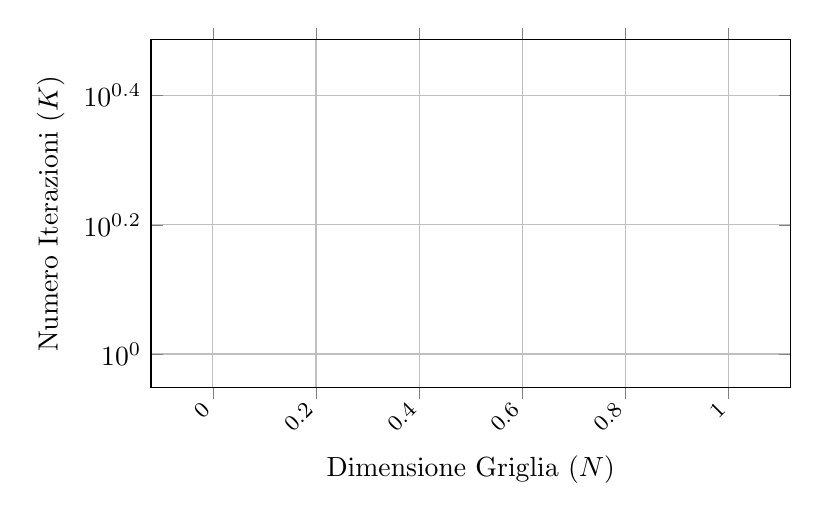
\begin{tikzpicture}
\begin{axis}[
    width=0.8\textwidth, height=6cm,
    xlabel={Dimensione Griglia ($N$)},
    ylabel={Numero Iterazioni ($K$)},
    xtick=data,
    x tick label style={/pgf/number format/1000 sep=, rotate=45, anchor=east, font=\footnotesize},
    grid=major,
    legend pos=north west,
    enlargelimits=0.12,
    ymode=log,
    log origin=infty,
    ymin=10,
    ybar,
    bar width=4pt,
]
    % Iterazioni Standard
    \addplot coordinates {\benchCoordIterStd};
    \addlegendentry{Standard}

    % Iterazioni In-Place
    \addplot coordinates {\benchCoordIterIp};
    \addlegendentry{In-Place}
\end{axis}
\end{tikzpicture}
\caption{Confronto delle iterazioni di convergenza ($K$) tra Standard e In-Place. Scala logaritmica sulle ordinate.}
\label{fig:iterazioni}
\end{figure}

\noindent
\textbf{Commento}: si osserva come l'aggiornamento \textit{In-Place} acceleri la convergenza nelle istanze con $N$ pari a \benchIstanzeKridotto{}, grazie alla propagazione immediata dei valori all'interno della stessa iterazione. Nelle istanze in cui i cicli si equivalgono ($N$ pari a \benchIstanzeKpari{}) la geometria costringe la funzione valore a propagarsi in verso opposto alla scansione per righe dei cicli \texttt{for}, annullando l'effetto a catena. Si noti inoltre che $K$ non cresce monotonamente con $N$: dipende dall'eccentricità del Goal, non dalla dimensione della griglia, come mostrato nella Tabella~\ref{tab:eccentricita}.

\clearpage
% 3. Grafico dell'Occupazione di Memoria Extra vs Teorico Theta(N^2)
\begin{figure}[htbp]
\centering
\begin{tikzpicture}
\begin{axis}[
    width=0.8\textwidth, height=6cm,
    xlabel={Dimensione Griglia ($N$)},
    ylabel={Memoria Extra (KB)},
    grid=major,
    legend pos=north west,
]
    % Standard Memoria
    \addplot [mark=*, red, thick] coordinates {\benchCoordMemStd};
    \addlegendentry{Standard (Misurato)}

    % Curva teorica Theta(N^2) per la memoria
    \addplot [domain=20:\benchNmax, samples=50, dashed, gray, thick]
        {\benchNormMem * (x/\benchNmax)^2};
    \addlegendentry{Teorico $\Theta(N^2)$}

    % In-Place Memoria
    \addplot [mark=square*, blue, thick] coordinates {\benchCoordMemIp};
    \addlegendentry{In-Place $\Theta(1)$}
\end{axis}
\end{tikzpicture}
\caption{Verifica sperimentale della complessità spaziale ausiliaria.}
\label{fig:memoria}
\end{figure}

\noindent
\textbf{Commento}: la sovrapposizione tra stima teorica e misura empirica è pressoché perfetta ($R^2 = \benchErreQuadMem{}$). La serie In-Place resta costantemente nulla, a conferma che la variante non alloca alcuna memoria ausiliaria proporzionale a $N$.

\clearpage
\subsection{Conclusioni}
L'analisi dei dati empirici permette di trarre le seguenti conclusioni sulle prestazioni dei due algoritmi:

\begin{enumerate}
    \item \textbf{Il numero di iterazioni è determinato dall'eccentricità del Goal}: la relazione $K_{\text{Standard}} = \text{ecc}(G) + 1$ è verificata esattamente su tutte e \benchNistanze{} le istanze. Ne consegue $K \le |\mathcal{S}| \le N^2$ e quindi il limite $O(N^4)$ per il caso peggiore, effettivamente avvicinato dalle istanze a corridoio unico ($N=120$, \benchKtop{} iterazioni).

    \item \textbf{Accelerazione della Convergenza}: Nelle istanze caratterizzate da percorsi orientati favorevolmente rispetto alla scansione ($N$ pari a \benchIstanzeKridotto{}) la variante \textbf{In-Place} riduce sensibilmente il numero di iterazioni: per $N=\benchNgrande{}$ i cicli scendono da \benchKstdGrande{} a \benchKipGrande{} ($-\benchRiduzioneGrande{}\%$). L'aggiornamento immediato degli stati consente al valore di propagarsi lungo più celle adiacenti già all'interno della medesima iterazione.

    \item \textbf{Impatto della Geometria degli Ostacoli}: Nelle istanze con $N$ pari a \benchIstanzeKpari{} entrambe le varianti richiedono lo stesso numero di cicli. Ciò accade quando i muri e i colli di bottiglia costringono la funzione valore a propagarsi in verso opposto rispetto a quello dei cicli \texttt{for}, rendendo inefficace l'effetto a catena dell'In-Place.

    \item \textbf{Efficienza Temporale}: L'algoritmo In-Place risulta più rapido dello Standard su tutte le istanze misurate. Il vantaggio è marcato dove riduce le iterazioni (per $N=\benchNgrande{}$ si passa da $\benchTempoGrandeStd{}\text{ ms}$ a $\benchTempoGrandeIp{}\text{ ms}$) e resta comunque presente altrove, poiché anche a parità di iterazioni la variante evita la copia della matrice $V_{old}$ a ogni ciclo.

    \item \textbf{Complessità Temporale}: Viene confermata la complessità teorica $\Theta(K \cdot N^2)$: l'esponente stimato per il costo di una singola iterazione vale $\benchAlfaTempoStd{}$ per la Standard e $\benchAlfaTempoIp{}$ per la In-Place, entrambi compatibili con $\Theta(N^2)$.

    \item \textbf{Complessità Spaziale}: Viene confermata la complessità spaziale teorica. La variante Standard scala quadraticamente ($\alpha = \benchAlfaMem{}$, $R^2 = \benchErreQuadMem{}$) fino a richiedere $\benchMemTop{}\text{ KB}$ di memoria ausiliaria per $N=\benchNtop{}$, mentre la variante In-Place lavora direttamente sulla matrice principale senza allocare nulla, verificando l'andamento $\Theta(1)$.
\end{enumerate}
